\section{Porte}
Sur l'image ci-dessous, la porte dans son état original :
\begin{figure}[H]
    \centering
    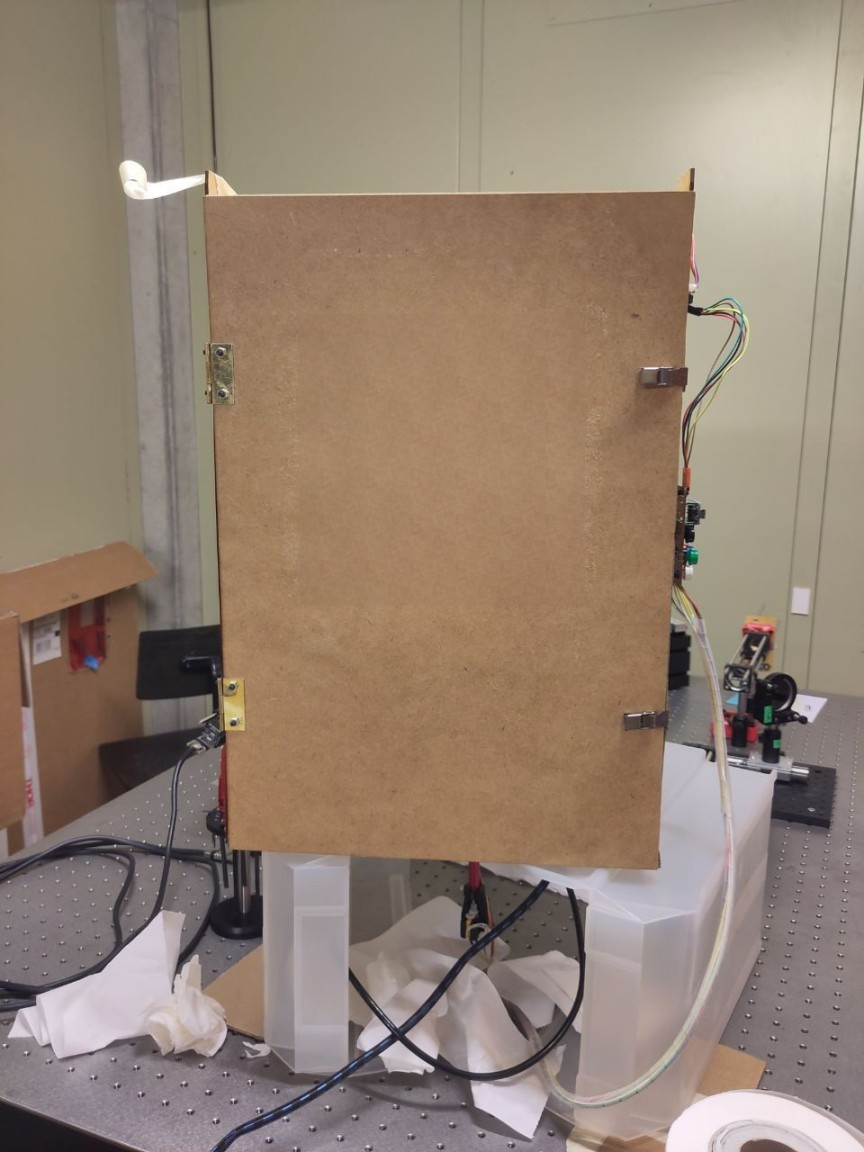
\includegraphics[width=0.5\textwidth]{assets/figures/ameliorations/porte_sans_fenetre.png}
    \caption{Photo de la porte avant modification}\label{photo porte}
\end{figure}

\newpage
Après une découpe dans le panneau de la porte, et le design de pièces de fixations et d'un chablon de perçage,
la porte est désormais équipée d'une fenetre:
\begin{figure}[H]
    \centering
    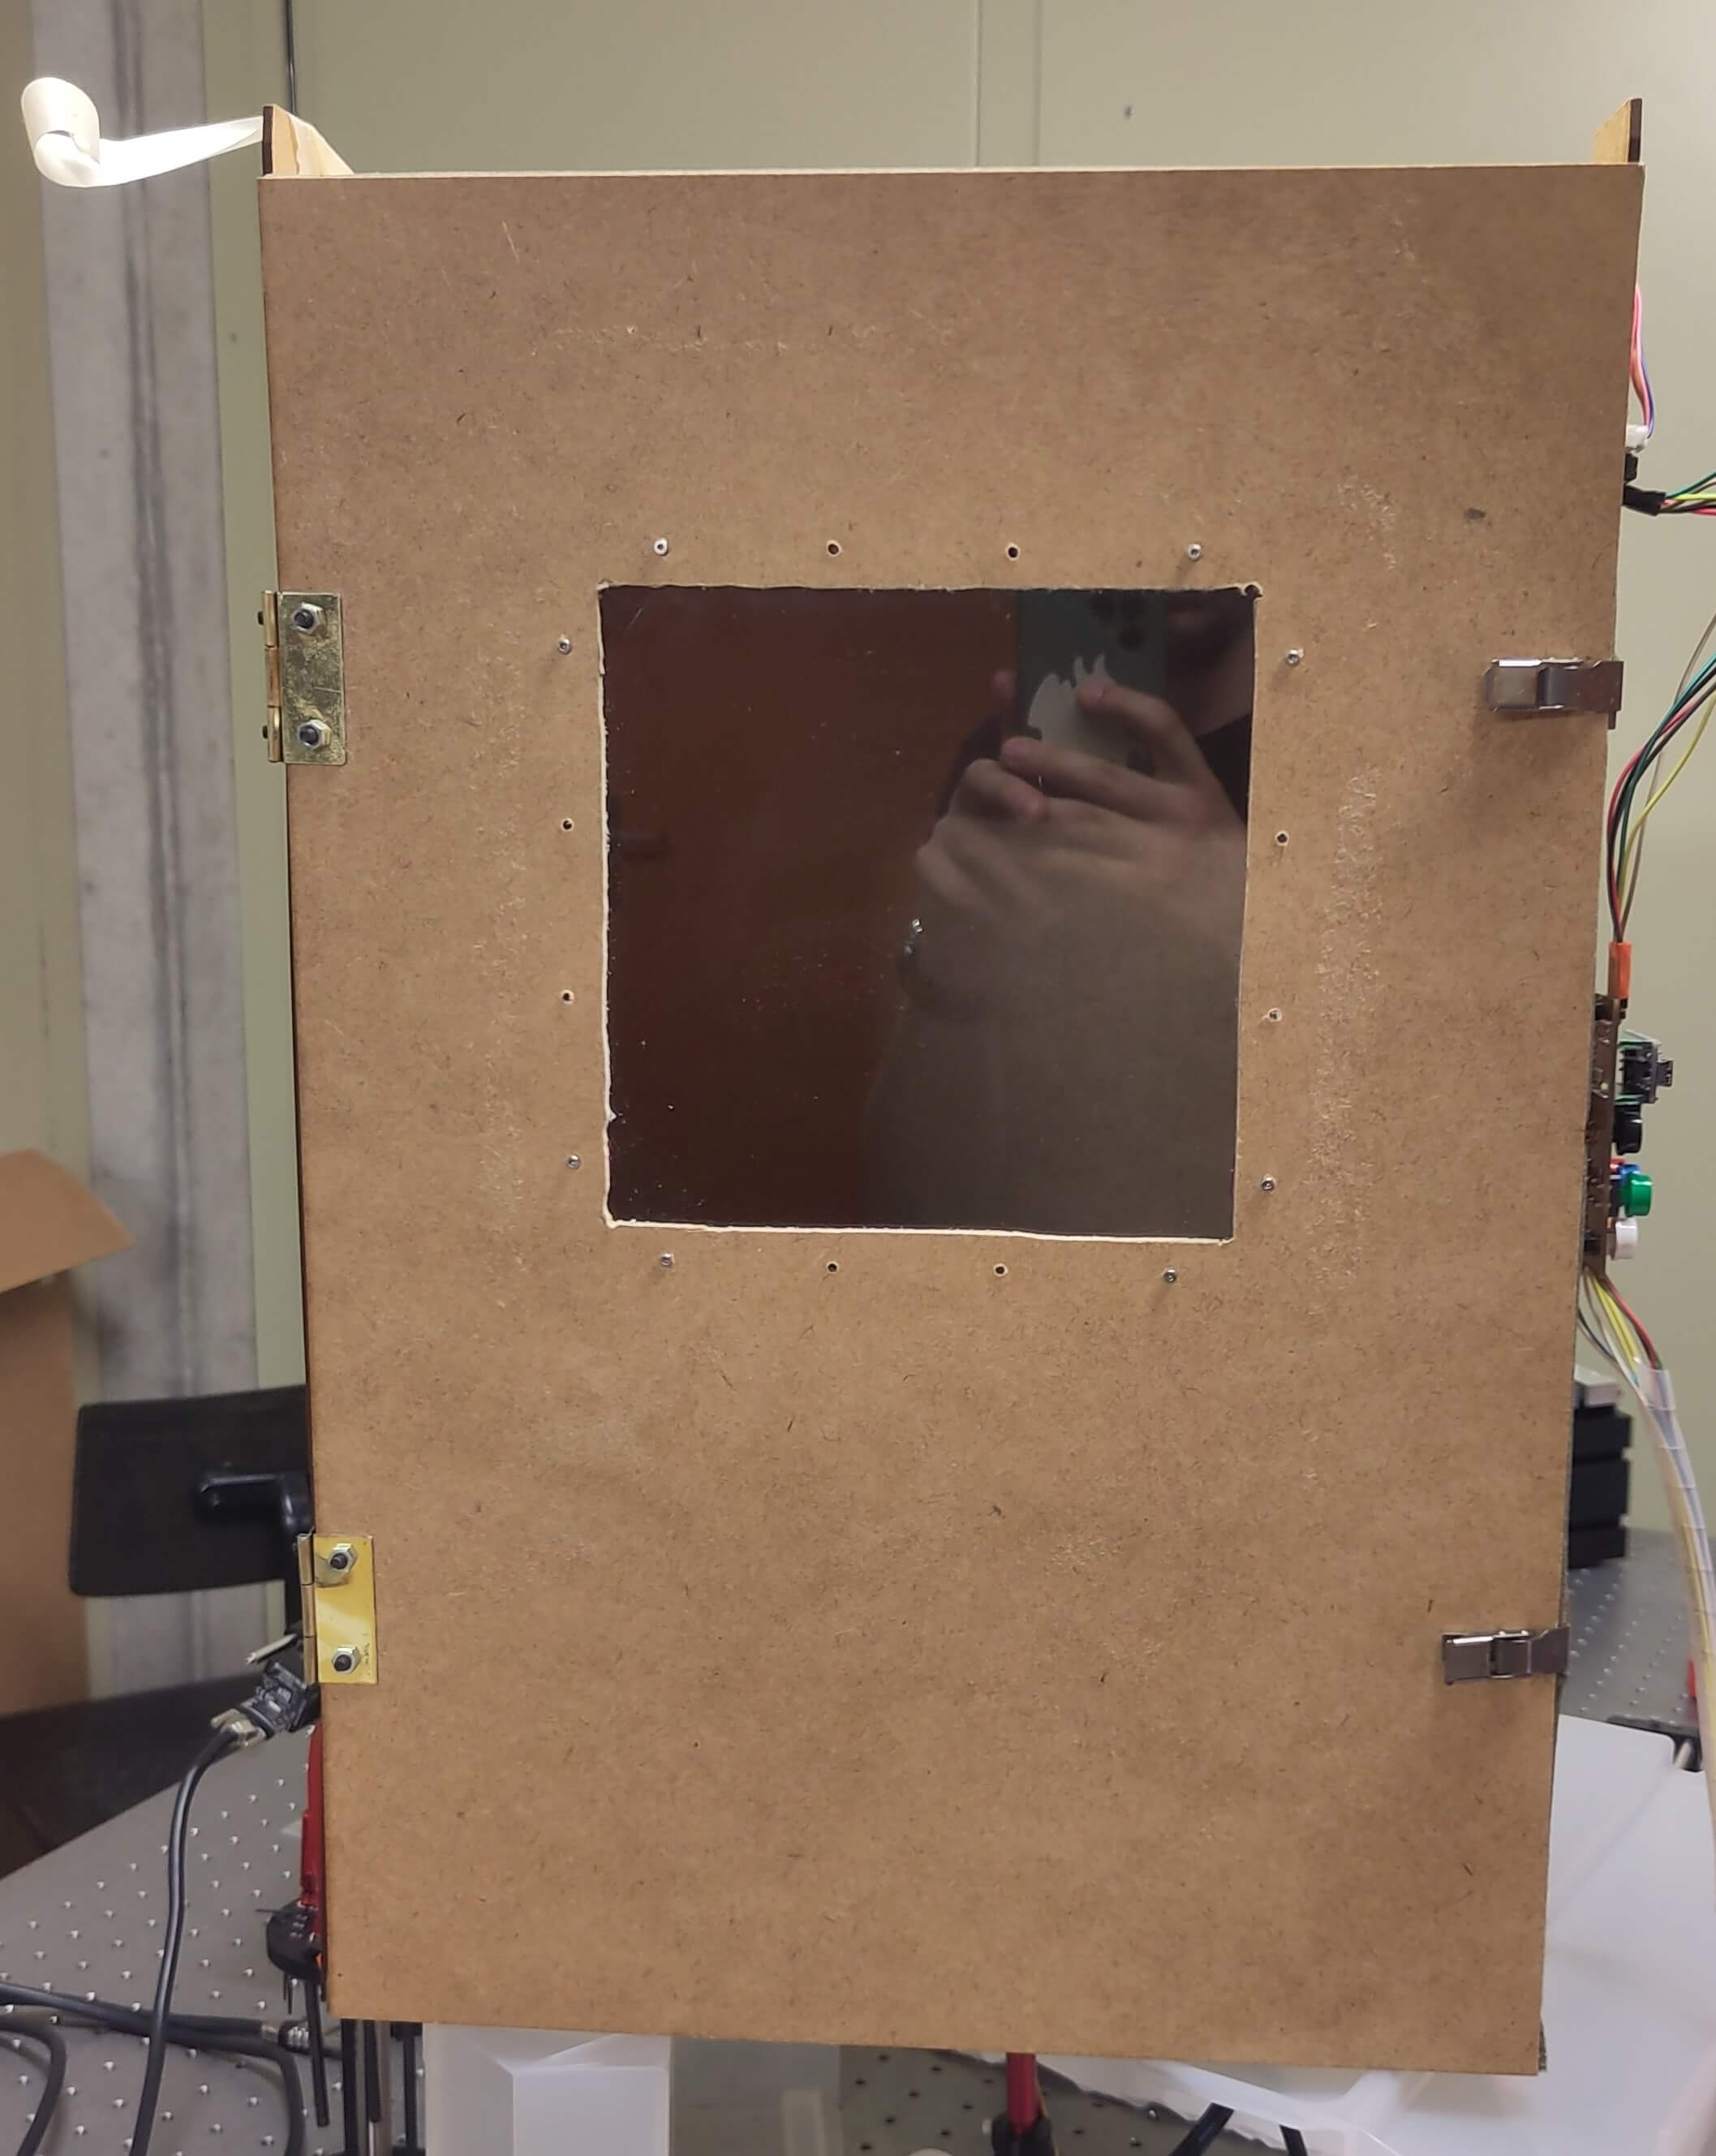
\includegraphics[width=0.5\textwidth]{assets/figures/ameliorations/porte_avec_fenetre.jpg}
    \caption{Photo de la porte après modification}\label{photo porte fenetre}
\end{figure}

DECRIRE FIXATION


\newpage
\section{Mesures}
\subsection{Problématique et situation d'origine}
Le procédé de mesure d'origine est sommaire et nécessite beaucoup de temps, en effet il convient de:
\begin{enumerate}
    \item Placer le disque dans le faisceau :
          \begin{figure}[H]
              \centering
              
\includegraphics[width=0.5\textwidth]{assets/figures/Placeholder.jpeg}
              \caption{Placeholder}\label{Placeholder}
          \end{figure}

    \item Attendre quelques secondes que la mesure sur le logiciel soit stable:
          \begin{figure}[H]
              \centering
              
\includegraphics[width=0.5\textwidth]{assets/figures/Placeholder.jpeg}
              \caption{Placeholder}\label{Placeholder}
          \end{figure}

    \item Prendre la mesure l'enregistrer en format \textbf{.csv} avec le numéro de mesure.
    \item Tourner le disque d'un petit angle:
          \begin{figure}[H]
              \centering
              
\includegraphics[width=0.5\textwidth]{assets/figures/Placeholder.jpeg}
              \caption{Placeholder}\label{Placeholder}
          \end{figure}
\end{enumerate}

Répéter en suite les étapes \textbf{2 à 4} pour autant de mesures qu'il le faut.
Dans le cadre de ce projet, plus il y a de données mieux c'est, il convient donc d'automatiser le
processus de prise de mesure au maximum pour pouvoir caractériser les écrans de turbulance facilement.

\subsection{Solution développée}
L'idée est de contrôler par ordinateur la prise de mesure ,interaction avec la caméra et la rotation de l'écran.
Après une petite configuration, l'utilisateur doit pouvoir laisser le système tourner et prendre les mesures nécessaires sans
interaction externe nécessaire.

\subsubsection{Caméra}

La caméra utilisée pour mesurer le front d'ondes est une \textbf{Thorlabs WFS40-7AR}:
\begin{figure}[H]
    \centering
    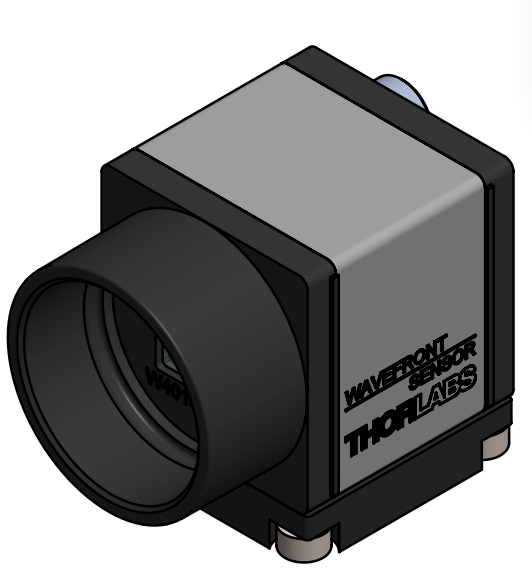
\includegraphics[width=0.4\textwidth]{assets/figures/ameliorations/thorlabs_40_7AR.png}
    \caption[Image de la caméra Thorlabs]{Image de la caméra Thorlabs \autocite{Camera_thorlabs_photo}}\label{fig:camera_thorlabs}
\end{figure}

Comme dit précédemment, il est possible d'intéragir avec la caméra à l'aide du logiciel fourni par Thorlabs, ce dernier permet de régler
la caméra, lire différentes mesures et visualiser le front d'onde.

La problématique était donc de trouver un moyen de communiquer avec la caméra, hors du logiciel dédié pour créer le programme de mesures.
Le manuel de la caméra, parle de la possibilité d'utiliser \textbf{LabView} pour accéder aux données et contrôler la caméra, en effet des
drivers spécifiques sont installés avec le programme de Thorlabs. Malheureusement cette solution ne fut pas retenue pour les raisons suivantes:

\begin{itemize}
    \item Le système de liscence de LabView à l'école est très contraignant.
    \item Mon système d'exploitation principal est MacOs (ainsi que celui de M. Jolissaint), LabView est peu compatible avec Mac et l'emulation de windows crash à cause des drivers.
\end{itemize}

Cela a donc porté mon regard sur l'utilisation de \textbf{Matlab}, et par chance, un utilisateur a développé une librairie Matlab permettant d'utiliser la caméra ! Cette ressource est disponible ici :
\url{https://www.mathworks.com/matlabcentral/fileexchange/116485-driver-for-thorlabs-shack-hartmann-wavefront-sensors-wfs}, elle a comme pré-requis, l'installation du logiciel de Thorlabs pour accéder aux drivers.

Il faut donc toujours utiliser un ordinateur sous windows, mais Matlab étant plus simple au niveau de ses liscences, il a été plus simple pour moi de juste travailler sur l'ordinateur du laboratoire.

\subsubsection{Rotation de l'écran}
Pour faire tourner l'écran il fallait :
\begin{itemize}
    \item Un moyen de faire tourner l'écran.
    \item Faire communiquer l'ordinateur et le moyen de rotation.
\end{itemize}

Pour répondre au 1er besoin, j'ai utilisé un moteur pas-à-pas \textbf{28byj-48} :
\begin{figure}[H]
    \centering
    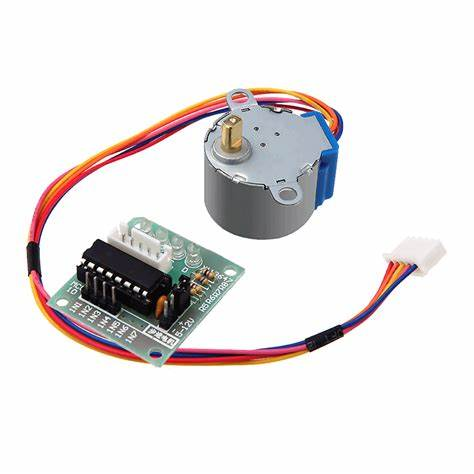
\includegraphics[width=0.5\textwidth]{assets/figures/ameliorations/stepper.jpeg}
    \caption[Moteur 28byj-48 pas-à-pas et son driver]{Moteur 28byj-48 pas-à-pas et son driver \autocite{photo_28byj-48}}
\end{figure}

\newpage
Pour la communication entre l'ordinateur et le driver du moteur, un arduino nano (clône) est utilisé :
\begin{figure}[H]
    \centering
    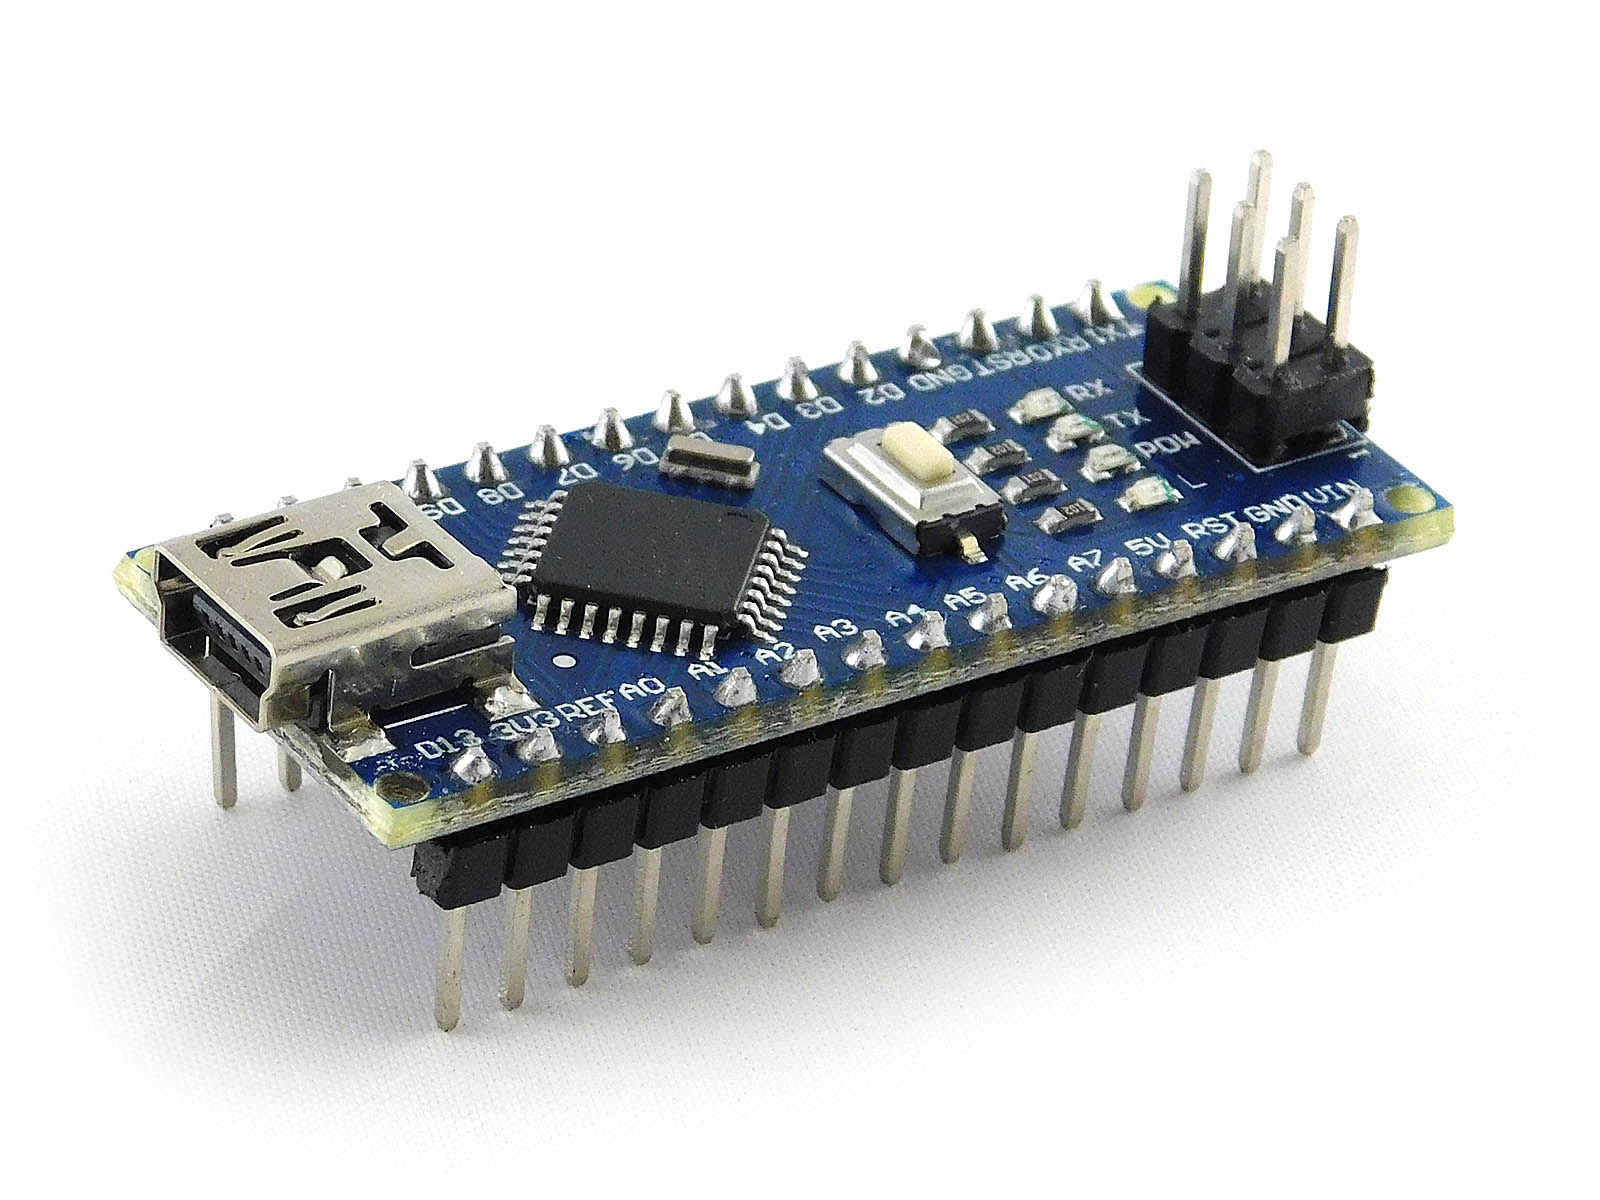
\includegraphics[width = 0.45\textwidth]{assets/figures/ameliorations/arduino_nano.jpg}
    \caption[Exemple de clône d'arduino nano]{Exemple de clône d'arduino nano \autocite{clone_nano}}
\end{figure}